\section{The network}

For the purpose of object recognition, we are deploying a  convolutional neural network, specifically designed for this thesis. During the training process, the network is fed images along with labels of the class. %To achieve a robust and balanced training dataset, we are generating synthetic images using starGen. Real images are later used to fine-tune the model. 
The validation process is used for determining the best-performing parameters of the network. The network is validated using both synthetic and real images.
After establishing the configuration of the model, the system is tested on real data.

\subsection{The architecture}

When designing the architecture of our network, we took inspiration from LeNet \cite{lenet5}. The model was designed to classify grey-scale images of handwritten digits, where the main indicators of each class are its morphological features. Images in our work are very similar and the difference between each class also relies on the object's morphological features, such as shape, density, etc. 

% prepisat este
The dimensions of the input data to the LeNet network are not consistent with the size of our data. As for this, the topology of the LeNet5 network needed some modifications, to be able to fit our input data. Some changes were made regarding the number of layers and the dimensions of kernels in convolutional layers. 

The topology of network is demonstrated in the Figure \ref{img:arch0} and consists of following layers: 

\begin{enumerate}
    \item \textbf{Layer C1} \\
    The first convolution layer consists of 6 kernels of size 5x5. The convolution operation is performed using a stride of 1 with zero padding on the image. The input to the layer is the grey-scale image of 50x50x1 and the output feature maps are of size 46x46, which makes the output volume 46x46x6. The layer has a total of 156 learnable parameters, including 150 weights and 6 biases. 
    
    \item \textbf{Layer S2} \\
    Subsampling layer that uses average pooling with a kernel of 2x2 size and stride of 2. The input volume to the layer is 46x46x6, and the pooling layer reduces the spatial size by a factor of 2, while the depth stays the same. This results in an output volume of 23x23x6.
    
    \item \textbf{Layer C3} \\
    The second convolution layer with 16 kernels of size 4x4, moving with a stride of 1 and zero padding on the input data. The output consists of 16 feature maps of size 20x20. The layer introduces 96 weights and 1 bias per filter, which is a total of 1552 learnable parameters.
    
    \item \textbf{Layer S4} \\
    The structure of the subsampling layer is the same as the layer S2. The input to the layer is a volume of 20x20x16 which makes the output 10x10x16.
    
    \item \textbf{Layer C5} \\
    The third convolution layer with 32 kernels of size 5x5. Again moving with a stride of 1 and zero padding. The layer outputs the volume 6x6x32. It has a total of 12 832 learnable parameters, with 400 weights and 1 bias per filter. 
    
    \item \textbf{Layer S6} \\
    The last subsampling layer, with the same structure as the previous ones. The layer receives the input volume of 6x6x32 and outputs 32 feature maps of size 3x3.
    
    \item \textbf{Layer C7} \\
    The last convolution layer consists of 120 3x3 convolution kernels, moving with a stride of 1 and zero padding on the input data. As the dimensions of the input data are the same as the convolution kernel, the output is one dimensional tensor with a length of 120. The layer has 289 parameters per filter, which results in a total of 34 680 learnable parameters. 
    
    \item \textbf{Layer F8} \\
    The first fully connected layer contains 84 neurons. The input to the layer is a tensor with a length of 120, or we can also imagine it as 120 neurons. Each neuron from the input is connected to each neuron in the layer. This makes a total of 10 080 connections, where each connection introduces one learnable weight. Each neuron in the layer also contains one bias value. This gives a total of 10 164 learnable parameters.
    
    \item \textbf{Layer F9} \\
    The second fully connected layer where the number of neurons is the number of classes. In the case of LeNet5, it was 10 but in our case, it's 6 neurons. Connecting with the previous layer with 84 neurons creates 504 weights and 6 biases, for a total of 510 learnable parameters. 
\end{enumerate}

The network is made up of 9 layers and has a total of 59 894 learnable parameters. It is standard practice for the topology to consist of alternating convolutional and pooling layers, followed by fully-connected layers at the end. 

Important to mention, that after each convolutional and fully-connected layer, non-linear activation is applied to the data. The specific choice of activation function is not mentioned here as it will be a hyperparameter determined by validation of the network. 


\begin{figure}[h]
    \centering
    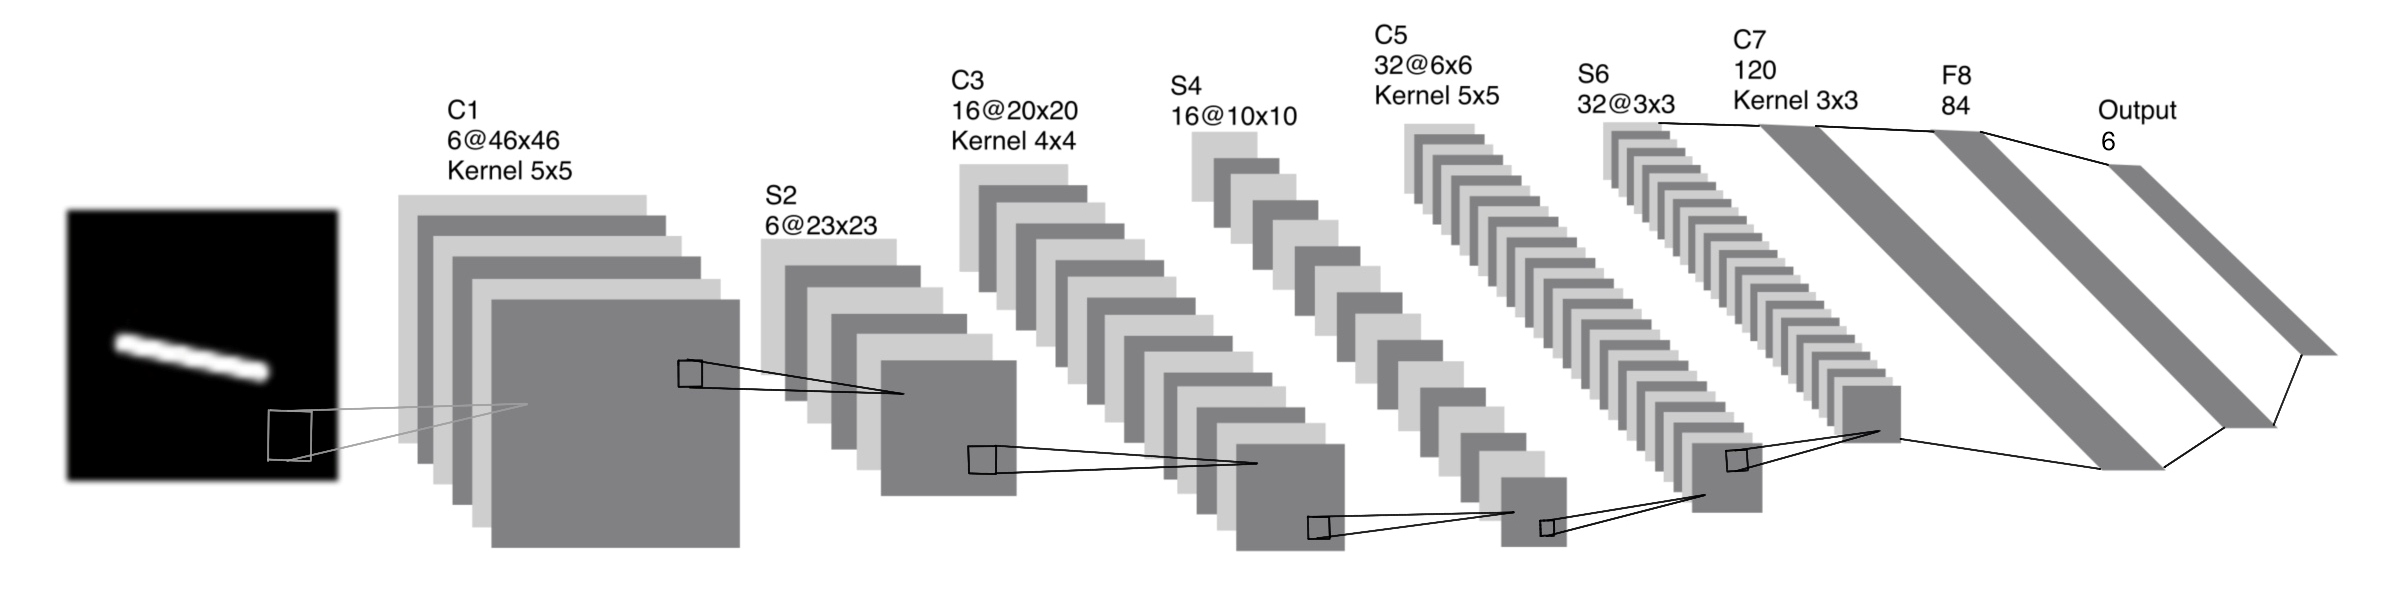
\includegraphics[width=\textwidth]{images/architectureCNN2.png}
    \caption[The proposed architecture of the neural network]
    {The proposed architecture of the neural network. 
    For each convolutional layer (denoted as “C”) the information about the kernel and size of output feature maps is defined (N@MxM, where N is the number of filters used and MxM is the spatial size of the feature maps). 
    Subsampling layers ("S") always operate with a 2x2 kernel and reduce only the spatial size of the feature maps. The output information is defined in the same way as with convolutional layers. 
    The last two layers of the network are fully connected ("F") and specify the number of neurons in the layer. The last fully-connected layer is denoted as the output layer.}
    \label{img:arch0}
\end{figure}

\subsection{Parameters} \label{sec:parametersNetwork}

% softmax na konci
% cross entropy na pocitanie gradientu
% early stopping pre val loss aj accuracy
% parametre optimizeru
% scheduler pre LR
% regularization, dropout
% augumentation
% activation function


During the training, images fed to the network come in batches, whose size is determined by parameter \textit{batch size}. Each batch of images is passed through the layers of the network. After each convolution layer, \textit{activation function} is applied to the output. Before the image is passed into the fully-connected layer, it must be flattened into a one-dimensional vector. The last fully-connected layer outputs the class scores of the image. \textit{Softmax activation} is applied to class scores to normalize them into class probabilities, where each value represents how sure our network is that the input is the specific class. A useful feature of softmax activation is that adding probability values for each class together outputs 1. 

\textit{Loss function} is used to measure the performance of the network. It consists of two components: data loss and regularization loss. Data loss calculates the quality of the prediction compared to ground truth labels, for which we use \textit{cross-entropy loss}. \textit{Regularization loss} is only the function of weights, and its goal is to penalize large weights.  

During backpropagation, \textit{optimizer} is used to update the weights of the network to minimize the loss function. The optimizer uses the gradient of the loss function to determine the direction toward the local minima. The size of the step we take in that direction is defined by parameter \textit{learning rate}.  Weights are updated after each pass of the batch through the network - one iteration. When all training data has passed through the network through batches, one \textit{epoch} has passed.

After each epoch, \textit{validation data} is used to determine the performance of our network. Validation loss is computed but it‘s not used to update weights during backpropagation. During the training process, validation loss is most commonly used to adjust the learning rate through \textit{scheduler}. After the network is trained, the performance on the validation data is key to adjusting the hyperparameters of the network to achieve better results. 

The network is trained for a certain number of epochs, which is a hyperparameter defined by the user. However, to avoid overfitting of data, \textit{early stopping algorithm} is deployed, which stops the process of training if needed.  

\subsubsection{Activation function}

Activation function is used for non-linearity in forward pass of the network. Function takes one number and performs defined mathematical operation on it. In our work we will be testing following activation functions:
\begin{itemize}
    \item \textit{Sigmoid activation}
        \begin{equation}
            \sigma (x) = \frac{1}{1 + e^{-x}}
        \end{equation}
        
    \item \textit{Hyperbolic tangent activation (tanh)}
        \begin{equation}
            tanh(x) = \frac{2}{1+e^{-2x}} - 1
        \end{equation}
    
    \item \textit{Rectified Linear Unit (RELU) activation}
        \begin{equation}
            f(x) = max(0,x)
        \end{equation}
        
    \item \textit{Leaky RELU activation}
        \begin{equation}
            f(x) = 
            \begin{cases}
                x,& \text{if } x\geq 0\\
                \alpha x ,& \text{otherwise}
            \end{cases}
        \end{equation}
\end{itemize}

Each activation has its advantages and disadvantages. Sigmoid was a very popular choice in the past as it was the closest approximation to the firing of the neuron in a biological sense. However, large negative and positive numbers get saturated, which results in a gradient close to zero. During backpropagation, this will kill the flow of the gradient and the network won't be able to learn. Another undesirable feature of the sigmoid is that it is not zero-centered which makes the gradient updates follow a zig-zag pattern. On the other hand tanh activation outputs zero-centered values but similar to sigmoid, large values get saturated. Nowadays, the most used activation is RELU activation. Positive numbers don't get saturated as they follow a linear path. Yet large gradient update of weights could cause the input values to RELU neurons to be always negative. This way the neuron always outputs zero, doesn't contribute to the learning process of the network and essentially "dies". One way to fix the problem is introduced by Leaky RELU. Instead of outputting zero when negative inputs come, the function multiplies the negative value with a small constant $\alpha$ \cite{standford}.

\subsubsection{Loss function}

The goal of training is to adjust the weights of the network so that during the forward pass the network achieves the highest accuracy on data. The update of weights is performed during backpropagation and is based on the value of the loss function. The loss function penalizes the poor performance of our network classification and weight configuration. It has the following form: 
\begin{equation}
    L = \frac{1}{N} \sum_{i=1}^{N} L_{i} + \lambda R(W)
\end{equation}
where the first part of the expression is data loss, and the second part is regularization loss. Data loss is calculated as the average loss over all samples in the batch, where the batch size is denoted as $N$. Regularization loss is computed from a set of weights $W$ and parameter $\lambda$ is a hyperparameter that represents the contribution of regularization loss $R(W)$ to the loss function $L$ \cite{standford}.

In our work, we use cross-entropy loss to calculate the data loss component. It is used to calculate the loss of the prediction when the output is a probability value ranging from 0 to 1. Using softmax activation in the last fully-connected layer transforms our class scores into probability values. The cross-entropy loss works in a way that it increases as the predicted value deviates from the actual class label and decreases when the value is closer to the truth. In our case, we are classifying into multiple classes and cross-entropy is therefore calculated for each class separately using the following formula: 

\begin{equation}
    L_i = - \sum_{c=1}^{M} y_c log(p_c)
\end{equation}

where $M$ is number of classes, $y_c$ is binary indicator that expresses if the class $c$ is correct classification for example $i$ and $p_c$ is predicted probability value that example $i$ is of class $c$ \cite{standford}.

However, even if we find the configuration of weights that can classify each example, various sets of weights can achieve the same result. To eliminate the ambiguity we want the network to have a preference for certain weights. This is achieved through regularization loss which penalizes certain types of weights. 

One of the most common types of regularization losses and the one we are using in our thesis is L2 regularization. It penalizes large weights as it is believed that smaller weights mean a simpler model. And keeping the model simple prevents overfitting on training data and generalizes better for unseen data. L2 regularization has the following form: 

\begin{equation}
    R(W) = \sum_{i}^N W_i ^ 2 
\end{equation}
where set of weight $W$ is defined as $W = w_1, w_2, ... w_N$ \cite{standford}.








\subsubsection{Optimizer}

We mentioned that the loss function is used to measure the performance of our model to adjust the weights accordingly. The tool that provides this update is an optimizer, which uses the output of the loss function to determine how to update the weights. More specifically it uses the gradient of the loss function to predict the direction of the steepest slope to find local minima of the loss function. How much we move in that direction is determined by the parameter learning rate, which is essential in optimization and very hard to determine. 
There are several types of optimizers and each uses a different method to optimize the weights. In our work we are implementing the following optimizers:
\begin{itemize}
    \item Stochastic Gradient Descend (SGD) with momentum 
    \item Root Mean Square Prop (RMSProp)
    \item Adaptive Moment Estimation (ADAM) 
\end{itemize}

SGD with momentum is one of the simpler optimizers. It uses the negative direction of the gradient as well as an accumulated gradient over past iterations, which imitates velocity. It has the following form: 

\begin{equation}
\begin{split}
    v_t = \beta \cdot v_{t-1} + g_t \\
    W_t = W_{t-1} + LR \cdot v_t
\end{split}
\end{equation}

where $v_t$ is weighted average of previous gradients, $\beta$ is hyper paramater called momentum which controls how much the previous gradients $v_{t-1}$ contribute to current $v_t$, $g_t$ is gradient, $W$ is weight vector and $LR$ is hyper parameter learning rate \cite{pytorchoptim}.

Another popular approach in optimizers is to use second order derivative of loss function instead of just using gradient. One of them is RMSProp which is defined as:

\begin{equation}
\begin{split}
    v_t = \alpha \cdot v_{t-1} + (1 - \alpha) \cdot g_t^2 \\
    W_t = W_{t-1} - LR \cdot g_t / (\sqrt{v_t} + \epsilon) 
\end{split}
\end{equation}

where $v$ is a weighted average of previous squares of gradients, $\alpha$ is a hyperparameter that controls how $v_t$ contributes to $v_{t+1}$, and $\epsilon$ is a small constant value that prevents division by zero. Similar to SGD with momentum, $g$ is the gradient, $W$ is the weight vector and $LR$ is the learning rate \cite{pytorchoptim}.

One of the most popular optimizers and one that is the most complex is ADAM. It utilizes ideas from both RMSProp and SGD with momentum. The update of weights looks as follows: 

\begin{equation}
\begin{split}
    m_t = \beta_1 \cdot m_{t-1} + (1 - \beta_1) \cdot g_t \\
    v_t = \beta_2 \cdot v_{t-1} + (1 - \beta_2) \cdot g_t^2 \\
    \hat{m_t} = m_t / (1 - \beta_1^t) \\
    \hat{v_t} = v_t / (1 - \beta_2^t) \\
    W_t = W_{t-1} - LR \cdot \hat{m_t} / (\sqrt{\hat{v_t}} + \epsilon) 
\end{split}
\end{equation}

where $m_t$ is weighted average of previous gradients, $v_t$ is weighted average of previous squares of gradients, $\beta_1$ and $\beta_2$ are hyper parameters and $\hat{m_t}$, $\hat{v_t}$ are corrected values to prevent bias towards zero. Other parameters are same as in the previous formulas \cite{pytorchoptim}.

\subsubsection{Scheduler}

Neural networks require a large number of hyperparameters to tune. Some of them don't affect the performance to such an extent while others are essential for the model to be set properly. One of such essential ones is the learning rate of optimizers. If it's too low the training process is excessively long. On the other hand, if we set it to be too large, the optimization diverges from the minima. It may also not be optimal for the learning rate to stay the same during the whole training process. When we are near the local minima, large steps could cause us to stray away from it, while in the beginning, it could help us reach the minima faster.
One of the ways to improve the optimization process is to use learning rate schedulers. There are several different types of schedulers. Some reduce the learning rate after each epoch, others reduce it after they have reached a certain epoch or after a given set of predefined epochs. The reduction may be done by multiplying the learning rate by some factor or the user defines the specific set of learning rates that will be used. One of the common ways is to use the validation loss to determine when to reduce the learning rate.

\subsubsection{Early stopping algorithm}
When the network is trained for a large number of epochs, it leads to overfitting of the training data. To eliminate this problem we are using an early stopping algorithm. During training, the algorithm watches how the validation loss evolves. If it starts to degrade and doesn't improve for a certain amount of time (patience) the training stops. The algorithm also remembers the model with the best performance and uses this as the final model.

\subsubsection{Dropout}
Another way to prevent the network from overfitting is to use dropout. It is a technique that randomly removes some neurons from the computation of the network. Each neuron is dropped randomly with the probability of p, which is a hyperparameter defined by the user. This allows the network to not rely on specific neurons, prevents layers from co-adaptation, and makes the model essentially more robust. The dropout can be applied to fully-connected layers as well as convolutional layers, but not to the output layer as this would remove prediction for a certain class \cite{standford}.

\subsubsection{Data augmentation }
One of the ways to improve the performance of the network is to have more data. In the real world, it is usually hard to obtain more labeled data for the training of the network. This problem is solved by data augmentation which essentially just uses the data we already have but modifies them in some way. With image data, augmentation usually involves rotation, flipping, scaling, cropping, color jitter, or adding noise. 
In our case data augmentation is not needed since we are generating synthetic images and have an unlimited amount of data. However, after training the network on synthetic data we are using real images to fine-tune the model. All the real images used in this thesis were hand-cropped by us and it took a significant amount of time. To increase the amount of data and in much less time, we are using some augmentation techniques. However, our data are prone to damage using some of the mentioned techniques. If we rotate the image, we may lose the astronomical object that was on the edge of the image. The same goes for cropping or scaling. Color jittering and noise addition are not suitable options as well as this would compromise the strictly defined profile of astronomical objects. For this reason, we are using only the following techniques: 

\begin{itemize}
    \item rotation by 90, 180, 270 degrees
    \item flipping vertically and horizontally
\end{itemize}








%%%%%%%%%%%%%%%%%%%%%%% alternatives %%%%%%%%%%%%%%
%However to find the minima, we need to move in the negative direction of the gradient.  While the gradient represents the steepest slope 

%The gradient of the loss function is computed over the whole batch of images. Using the optimizer, 

% there are several types of optimizer, and each have different parameters. 

%Learning rate determines the speed of the optimalization. 
%Optimizer uses the gradient of the loss function to determine the direction of steepest decrease to minimize the loss.

%the goal of the optimizer is to find a set of weights that minimizes the loss function. The gradient of the loss function is calculated to determine the direction of the steepest increase. 

% The network usually has a predefined number of epochs,


